
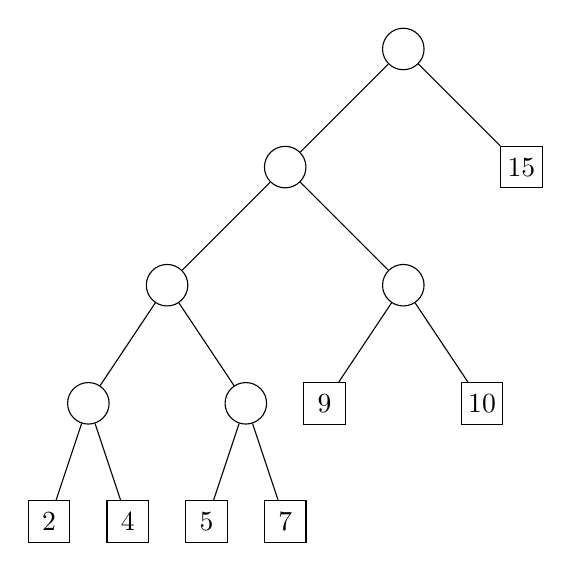
\begin{tikzpicture}[every node/.style={circle,draw},level 1/.style={sibling distance=30mm},level 2/.style={sibling distance=30mm},level 3/.style={sibling distance=20mm},level 4/.style={sibling distance=10mm},minimum size=0.50cm,iv/.style={draw,rectangle,minimum size=15pt,inner
sep=0pt,text=black},ev/.style={draw,circle,minimum
size=15pt,inner sep=0pt,text=black}]
\node[ev]{}
  child {node[ev]{}
         child {node[ev]{}
               child {node[ev]{}
               child {node[iv]{$2$}}
               child {node[iv]{$4$}}}
               child{node[ev]{}
                    child {node[iv]{$5$}}
                    child {node[iv]{$7$}}}
               }
         child {node[ev]{}
              child {node[iv]{$9$}}
              child {node[iv]{$10$}}}}
  child {node[iv]{$15$}
        child[missing]};
 
\end{tikzpicture}




